% Таблиці й рисунки з результатів; інтерпретацію додано після завершення перегляду.
\section{Результати}\label{sec:results}
% Generated from primary=gemini_reviewed; see ../manifest.json for source SHA-256.
\newif\ifpaperlatency
\paperlatencytrue
\newif\ifpaperindexing
\paperindexingtrue
\newif\ifpapergguf
\papergguftrue
\newif\ifpaperann
\paperanntrue
\newif\ifpaperfield
\paperfieldtrue
\newif\ifpaperextension
\paperextensiontrue
\newif\ifpaperextensionunique
\paperextensionuniquetrue


\subsection{Пошук і стійкість до вибору судді}
Таблиця~\ref{tab:retrieval} містить усі десять систем на однаковому наборі запитів із відповіддю. Довірчі інтервали описують варіацію за запитами за наведених міток, але не невизначеність самих міток. Таблиця~\ref{tab:judge-sensitivity} та рисунок~\ref{fig:judge-sensitivity} зберігають початкові й переглянутий варіанти. Перегляд виконує та сама модель Gemini; Gemini та Gemma мають спільного постачальника.

E5 має найвище середнє nDCG@10 за всіма трьома основними варіантами релевантності. Її перевага над adaptive не досягає порога 0,05 після поправки Holm за жодного варіанта; це не доводить еквівалентності. Adaptive перевершує обидва варіанти BM25 за основною метрикою після корекції, але статистично виявленої переваги над окремою EG2 або RRF немає. Вимкнення переранжування фраз не змінює оцінених метрик; відмінності інших абляцій адаптивної системи за nDCG@10 малі й статистично не виявлені на цьому наборі запитів. Ці результати не підтверджують загального твердження про перевагу адаптивного злиття над пошуком лише за векторами.

Лематизація підвищує середнє nDCG@10 BM25 за всіх трьох варіантів. Окремо наведене парне морфологічне порівняння підтримує різницю за початковими та переглянутими оцінками Gemini, тоді як за оцінками Gemma~4 12B інтервал охоплює нуль. Отже, сила висновку про морфологію залежить від оцінювання релевантності. Перегляд тією самою моделлю змінює 334 із 5\,572 початкових оцінок Gemini; усі 4\,481 початково узгоджені пари зберігаються.

\begin{table}[p]
\centering
\caption{Пошук документів за 170 запитами із відповіддю. Середні та 95\% бутстреп-інтервали за запитами відповідають оцінкам Gemini після перегляду розбіжностей тією самою моделлю. Дві частини зберігають усі п'ять метрик. Знак \textdagger{} позначає парну різницю з adaptive за скоригованого Holm $p<0.05$, не обов'язково поліпшення. R@100 визначено відносно пулу. E5 має менший текстовий набір кандидатів.}
\label{tab:retrieval}
% Generated from primary=gemini_reviewed; see ../manifest.json for source SHA-256.
% Means with 95% bootstrap CI; n=170. R@100 is pool-relative under incomplete judgments. Significance: paired comparison against adaptive only, \(p_{\mathrm{Holm}}<0.05\).
\begingroup\small\setlength{\tabcolsep}{4pt}\renewcommand{\arraystretch}{1.3}
\noindent\begin{tabularx}{\linewidth}{@{}l*{3}{>{\centering\arraybackslash}X}@{}}
\toprule
Система & nDCG@10 & R@100\textsuperscript{pool} & RR@10 \\
\midrule
bm25\_plain & \shortstack{0.450\textsuperscript{\textdagger} \\ {\footnotesize[0.413, 0.487]}} & \shortstack{0.648\textsuperscript{\textdagger} \\ {\footnotesize[0.611, 0.685]}} & \shortstack{0.738\textsuperscript{\textdagger} \\ {\footnotesize[0.682, 0.790]}} \\
bm25\_lemma & \shortstack{0.482\textsuperscript{\textdagger} \\ {\footnotesize[0.446, 0.518]}} & \shortstack{0.724\textsuperscript{\textdagger} \\ {\footnotesize[0.693, 0.755]}} & \shortstack{0.753\textsuperscript{\textdagger} \\ {\footnotesize[0.701, 0.802]}} \\
dense\_eg2 & \shortstack{0.633 \\ {\footnotesize[0.601, 0.664]}} & \shortstack{0.911 \\ {\footnotesize[0.890, 0.930]}} & \shortstack{0.872 \\ {\footnotesize[0.832, 0.910]}} \\
dense\_e5 & \shortstack{0.674 \\ {\footnotesize[0.647, 0.700]}} & \shortstack{0.880 \\ {\footnotesize[0.853, 0.906]}} & \shortstack{0.927 \\ {\footnotesize[0.894, 0.956]}} \\
rrf & \shortstack{0.630 \\ {\footnotesize[0.601, 0.660]}} & \shortstack{0.960\textsuperscript{\textdagger} \\ {\footnotesize[0.946, 0.972]}} & \shortstack{0.873 \\ {\footnotesize[0.835, 0.910]}} \\
adaptive & \shortstack{0.629 \\ {\footnotesize[0.596, 0.660]}} & \shortstack{0.908 \\ {\footnotesize[0.887, 0.928]}} & \shortstack{0.866 \\ {\footnotesize[0.826, 0.905]}} \\
adaptive-phrase & \shortstack{0.629 \\ {\footnotesize[0.596, 0.660]}} & \shortstack{0.908 \\ {\footnotesize[0.887, 0.928]}} & \shortstack{0.866 \\ {\footnotesize[0.826, 0.905]}} \\
adaptive-ident & \shortstack{0.629 \\ {\footnotesize[0.597, 0.661]}} & \shortstack{0.912 \\ {\footnotesize[0.892, 0.931]}} & \shortstack{0.866 \\ {\footnotesize[0.826, 0.905]}} \\
adaptive-short & \shortstack{0.629 \\ {\footnotesize[0.597, 0.660]}} & \shortstack{0.908 \\ {\footnotesize[0.887, 0.928]}} & \shortstack{0.866 \\ {\footnotesize[0.826, 0.905]}} \\
dense\_eg2\_256 & \shortstack{0.611 \\ {\footnotesize[0.577, 0.643]}} & \shortstack{0.888\textsuperscript{\textdagger} \\ {\footnotesize[0.863, 0.911]}} & \shortstack{0.873 \\ {\footnotesize[0.830, 0.913]}} \\
\bottomrule
\end{tabularx}\endgroup

\par\medskip
% Means with 95% bootstrap CI; n=170. R@100 is pool-relative under incomplete judgments. Significance: paired comparison against adaptive only, \(p_{\mathrm{Holm}}<0.05\).
\begingroup\small\setlength{\tabcolsep}{4pt}\renewcommand{\arraystretch}{1.3}
\noindent\begin{tabularx}{\linewidth}{@{}l*{2}{>{\centering\arraybackslash}X}@{}}
\toprule
Система & Success@1 & Success@5 \\
\midrule
bm25\_plain & \shortstack{0.635\textsuperscript{\textdagger} \\ {\footnotesize[0.559, 0.706]}} & \shortstack{0.876\textsuperscript{\textdagger} \\ {\footnotesize[0.824, 0.924]}} \\
bm25\_lemma & \shortstack{0.624\textsuperscript{\textdagger} \\ {\footnotesize[0.547, 0.694]}} & \shortstack{0.929 \\ {\footnotesize[0.888, 0.965]}} \\
dense\_eg2 & \shortstack{0.794 \\ {\footnotesize[0.729, 0.853]}} & \shortstack{0.971 \\ {\footnotesize[0.941, 0.994]}} \\
dense\_e5 & \shortstack{0.876 \\ {\footnotesize[0.824, 0.924]}} & \shortstack{0.988 \\ {\footnotesize[0.971, 1.000]}} \\
rrf & \shortstack{0.788 \\ {\footnotesize[0.724, 0.847]}} & \shortstack{0.976 \\ {\footnotesize[0.953, 0.994]}} \\
adaptive & \shortstack{0.782 \\ {\footnotesize[0.718, 0.841]}} & \shortstack{0.971 \\ {\footnotesize[0.941, 0.994]}} \\
adaptive-phrase & \shortstack{0.782 \\ {\footnotesize[0.718, 0.841]}} & \shortstack{0.971 \\ {\footnotesize[0.941, 0.994]}} \\
adaptive-ident & \shortstack{0.782 \\ {\footnotesize[0.718, 0.841]}} & \shortstack{0.971 \\ {\footnotesize[0.941, 0.994]}} \\
adaptive-short & \shortstack{0.782 \\ {\footnotesize[0.718, 0.841]}} & \shortstack{0.971 \\ {\footnotesize[0.941, 0.994]}} \\
dense\_eg2\_256 & \shortstack{0.818 \\ {\footnotesize[0.759, 0.871]}} & \shortstack{0.953 \\ {\footnotesize[0.918, 0.982]}} \\
\bottomrule
\end{tabularx}\endgroup

\par\smallskip
{\footnotesize \textdagger: p\textsubscript{Holm}<0.05, adaptive; R@100: відносно пулу.}

\end{table}

\begin{table}[p]
\centering
\caption{Стійкість nDCG@10 до оцінювання релевантності. Початкові оцінки Gemini та Gemma~4 12B збережено; варіант після перегляду змінює лише їхні розбіжності. Усі варіанти використовують ті самі зафіксовані прогони та 170 запитів. Оцінки GPT до цього порівняння не входять.}
\label{tab:judge-sensitivity}
% Generated from primary=gemini_reviewed; see ../manifest.json for source SHA-256.
% nDCG@10 with 95% bootstrap CI. Gemini reviewed is a within-model review. Gemini/Gemma12 share a provider family. No GPT or E4B in this principal comparison.
\begingroup\small\setlength{\tabcolsep}{4pt}\renewcommand{\arraystretch}{1.3}
\noindent\begin{tabularx}{\linewidth}{@{}l*{3}{>{\centering\arraybackslash}X}@{}}
\toprule
Система & Gemini початкові & Gemma12 початкові & Gemini переглянуті \\
\midrule
bm25\_plain & \shortstack{0.453 \\ {\footnotesize[0.416, 0.491]}} & \shortstack{0.500 \\ {\footnotesize[0.462, 0.536]}} & \shortstack{0.450 \\ {\footnotesize[0.413, 0.487]}} \\
bm25\_lemma & \shortstack{0.489 \\ {\footnotesize[0.453, 0.526]}} & \shortstack{0.519 \\ {\footnotesize[0.482, 0.554]}} & \shortstack{0.482 \\ {\footnotesize[0.446, 0.518]}} \\
dense\_eg2 & \shortstack{0.644 \\ {\footnotesize[0.613, 0.674]}} & \shortstack{0.681 \\ {\footnotesize[0.652, 0.709]}} & \shortstack{0.633 \\ {\footnotesize[0.601, 0.664]}} \\
dense\_e5 & \shortstack{0.685 \\ {\footnotesize[0.657, 0.711]}} & \shortstack{0.698 \\ {\footnotesize[0.671, 0.725]}} & \shortstack{0.674 \\ {\footnotesize[0.647, 0.700]}} \\
rrf & \shortstack{0.641 \\ {\footnotesize[0.612, 0.669]}} & \shortstack{0.665 \\ {\footnotesize[0.636, 0.694]}} & \shortstack{0.630 \\ {\footnotesize[0.601, 0.660]}} \\
adaptive & \shortstack{0.639 \\ {\footnotesize[0.608, 0.669]}} & \shortstack{0.675 \\ {\footnotesize[0.647, 0.703]}} & \shortstack{0.629 \\ {\footnotesize[0.596, 0.660]}} \\
adaptive-phrase & \shortstack{0.639 \\ {\footnotesize[0.608, 0.669]}} & \shortstack{0.675 \\ {\footnotesize[0.647, 0.703]}} & \shortstack{0.629 \\ {\footnotesize[0.596, 0.660]}} \\
adaptive-ident & \shortstack{0.639 \\ {\footnotesize[0.608, 0.669]}} & \shortstack{0.676 \\ {\footnotesize[0.648, 0.704]}} & \shortstack{0.629 \\ {\footnotesize[0.597, 0.661]}} \\
adaptive-short & \shortstack{0.639 \\ {\footnotesize[0.608, 0.669]}} & \shortstack{0.675 \\ {\footnotesize[0.647, 0.703]}} & \shortstack{0.629 \\ {\footnotesize[0.597, 0.660]}} \\
dense\_eg2\_256 & \shortstack{0.622 \\ {\footnotesize[0.589, 0.654]}} & \shortstack{0.665 \\ {\footnotesize[0.633, 0.696]}} & \shortstack{0.611 \\ {\footnotesize[0.577, 0.643]}} \\
\bottomrule
\end{tabularx}\endgroup

\end{table}

\begin{figure}[p]
\centering
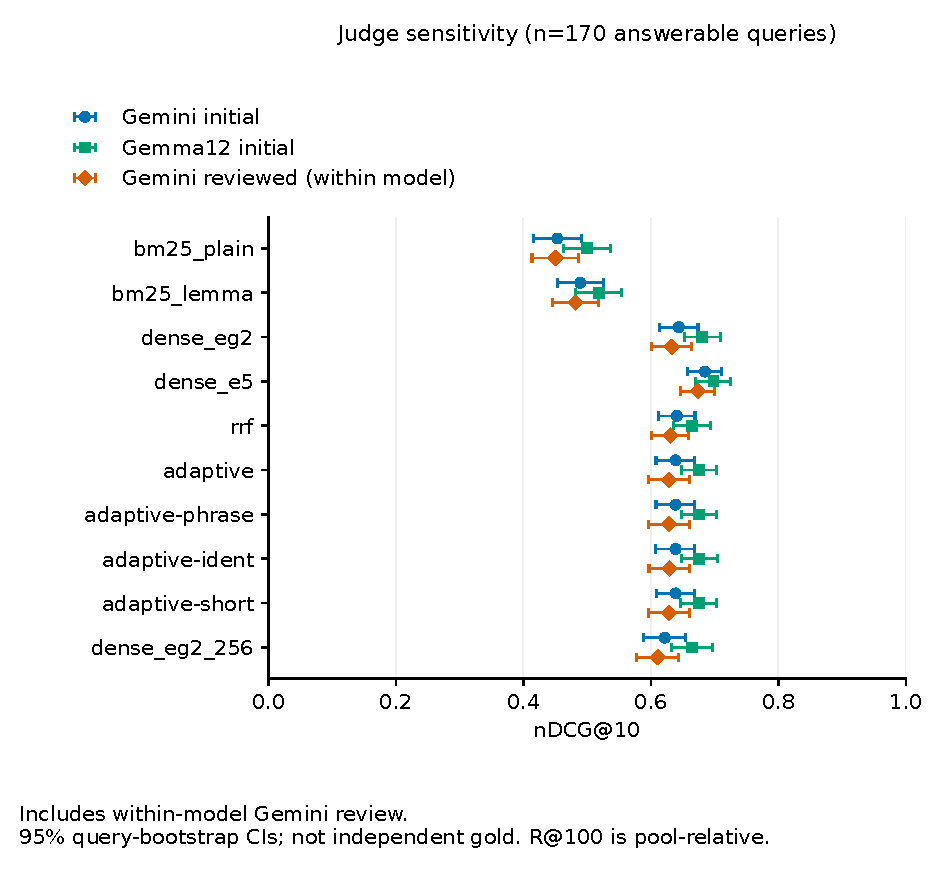
\includegraphics[width=\linewidth]{judge_sensitivity.pdf}
\caption{Метрики систем і 95\% бутстреп-інтервали за запитами для різних варіантів релевантності. Порівняння окремих інтервалів не замінює парних статистичних тестів.}
\label{fig:judge-sensitivity}
\end{figure}

\begin{figure}[p]
\centering
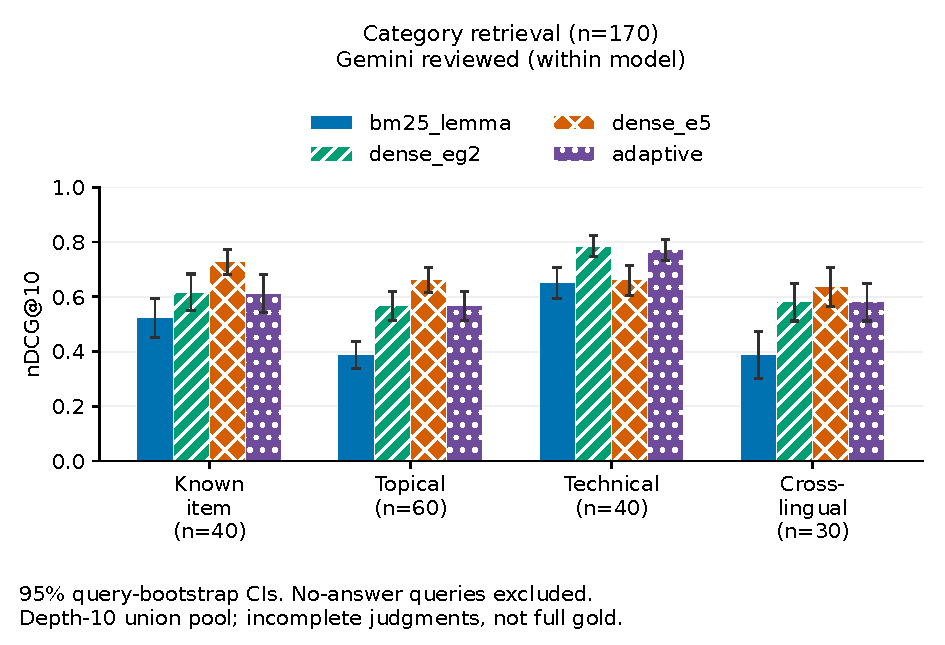
\includegraphics[width=\linewidth]{category_ndcg.pdf}
\caption{nDCG@10 за категоріями запитів для чотирьох основних систем за основного варіанта релевантності. Кожна категорія має власний бутстреп-інтервал. Запити без відповіді виключено.}
\label{fig:categories}
\end{figure}

\subsection{Контролі}
\paragraph{Множина кандидатів.} E5 шукає серед 4\,137 текстових документів; повний індекс EG2 містить 6\,054 документи, зокрема медіа. Обмеження EG2 тими самими 4\,137 текстовими документами (\sys{dense\_eg2\_text}) змінює його nDCG@10 на $-0{,}0015$ з переглянутими мітками Gemini (з 0,633 до 0,631); 0,29\% документів його першої десятки не було в оціненому пулі. Парна різниця EG2$_{\mathrm{text}}-{}$E5 становить $-0{,}042$ nDCG@10 (95\% ДІ від $-0{,}078$ до $-0{,}006$, некоригований $p=0{,}018$) з переглянутими мітками Gemini і $-0{,}019$ (від $-0{,}052$ до $0{,}014$, $p=0{,}26$) з мітками Gemma~4 12B (табл.~\ref{tab:encoder-control}). Отже, обмеження кандидатів мало змінює точкову оцінку в цьому контролі, а статистична підтримка різниці енкодерів залежить від міток. Ці дослідницькі порівняння мають некориговані p-значення та неповний пул оцінок.

\begin{table}[p]
\centering
\caption{E5 проти EG2 на тих самих 4\,137 текстових документах. $\Delta$ --- парна різниця від E5 з 95\% бутстреп-інтервалом за запитами і некоригованим $p$ знакового перестановкового тесту; неоцінені документи вважаються нерелевантними, їхню частку подано.}
\label{tab:encoder-control}
% Generated from primary=gemini_reviewed; see ../manifest.json for source SHA-256.
\noindent\textbf{Gemini reviewed}
\par\smallskip
% E5 against EG2 on the same 4137 text documents; source encoder_control.json
\begingroup\small\setlength{\tabcolsep}{4pt}\renewcommand{\arraystretch}{1.3}
\noindent\begin{tabularx}{\linewidth}{@{}l*{4}{>{\centering\arraybackslash}X}@{}}
\toprule
Система & nDCG@10 & $\Delta$ [95\% ДІ] vs E5 & p & Неоцінені@10 \\
\midrule
\sys{dense\_e5} & 0.674 & -- & -- & 0.000 \\
\sys{dense\_eg2} & 0.633 & \shortstack{-0.041 \\ {\footnotesize[-0.077, -0.005]}} & 0.023 & 0.000 \\
\sys{dense\_eg2\_text} & 0.631 & \shortstack{-0.042 \\ {\footnotesize[-0.078, -0.006]}} & 0.018 & 0.003 \\
\bottomrule
\end{tabularx}\endgroup

\par\medskip
\noindent\textbf{Gemini initial}
\par\smallskip
% E5 against EG2 on the same 4137 text documents; source encoder_control.json
\begingroup\small\setlength{\tabcolsep}{4pt}\renewcommand{\arraystretch}{1.3}
\noindent\begin{tabularx}{\linewidth}{@{}l*{4}{>{\centering\arraybackslash}X}@{}}
\toprule
Система & nDCG@10 & $\Delta$ [95\% ДІ] vs E5 & p & Неоцінені@10 \\
\midrule
\sys{dense\_e5} & 0.685 & -- & -- & 0.000 \\
\sys{dense\_eg2} & 0.644 & \shortstack{-0.041 \\ {\footnotesize[-0.075, -0.007]}} & 0.020 & 0.000 \\
\sys{dense\_eg2\_text} & 0.642 & \shortstack{-0.042 \\ {\footnotesize[-0.077, -0.009]}} & 0.014 & 0.003 \\
\bottomrule
\end{tabularx}\endgroup

\par\medskip
\noindent\textbf{Gemma 12B initial}
\par\smallskip
% E5 against EG2 on the same 4137 text documents; source encoder_control.json
\begingroup\small\setlength{\tabcolsep}{4pt}\renewcommand{\arraystretch}{1.3}
\noindent\begin{tabularx}{\linewidth}{@{}l*{4}{>{\centering\arraybackslash}X}@{}}
\toprule
Система & nDCG@10 & $\Delta$ [95\% ДІ] vs E5 & p & Неоцінені@10 \\
\midrule
\sys{dense\_e5} & 0.698 & -- & -- & 0.000 \\
\sys{dense\_eg2} & 0.681 & \shortstack{-0.018 \\ {\footnotesize[-0.050, +0.015]}} & 0.285 & 0.000 \\
\sys{dense\_eg2\_text} & 0.680 & \shortstack{-0.019 \\ {\footnotesize[-0.052, +0.014]}} & 0.258 & 0.003 \\
\bottomrule
\end{tabularx}\endgroup

\end{table}

\paragraph{Покриття цілими словами.} Перевірка точної фрази в адаптивному правилі рахувала підрядки (додаток~\ref{sec:intro-history}). З виправленим правилом перша десятка змінюється для одного запиту з 200 у кожному адаптивному варіанті, а nDCG@10 адаптивної системи змінюється з 0,629 до 0,627 (переглянуті Gemini), з 0,639 до 0,637 (початкові Gemini) і лишається 0,675 (Gemma~4 12B). Зафіксовані основні результати збережено; виправлена точкова оцінка не створює переваги адаптивного методу над щільним EG2.

\subsection{Судді}
Табл.~\ref{tab:judge-checks} показує оцінки на всьому пулі та на двох підмножинах із очікуваннями, заданими побудовою: цільових документах у пулі й парах запитів, позначених безвідповідними. Ці очікування не є незалежними людськими мітками. Табл.~\ref{tab:judge-agreement} подає попарну узгодженість. Gemini, дві моделі Gemma і GPT-6-Luna узгоджуються з лінійно зваженою $\kappa$ від 0,535 до 0,652. Gemini ставить оцінку~2 цільовому документу запиту з відповіддю у 85,8\% зі 134 цілей у пулі, Gemma~4 12B --- у 67,2\%: більша модель Gemma загалом найкраще узгоджується з Gemini, але рідко ставить повний бал. На 708 парах запитів без відповіді Gemini, Gemma~4 12B і Gemma~4 E4B ставлять 0 у 90,4\%, 91,2\% і 93,5\% пар.

GPT-6-Luna, яка писала запити, --- найпоблажливіший суддя: її середня оцінка 0,633 проти 0,421--0,447 в інших суддів, і вона ставить додатну оцінку 24,3\% пар запитів без відповіді проти 6,5--9,6\% в інших. Її оцінки в середньому на 0,19--0,21 вищі, ніж у кожного іншого судді. Це узгоджується із самопреференцією автора запитів, але загальна поблажливість дала б ту саму картину. Наявне порівняння не розрізняє цих пояснень. Оцінки GPT не входять до жодних міток релевантності.

\begin{table}[p]
\centering
\caption{Судді на 5\,572 парах пулу: середня оцінка, кількість оцінок і перевірки за побудовою (частка цілей запитів з відповіддю в пулі з оцінкою 2; частка пар запитів без відповіді з оцінкою 0).}
\label{tab:judge-checks}
% Generated from primary=gemini_reviewed; see ../manifest.json for source SHA-256.
% grades on the whole pool and known-answer checks; source judges.json
\begingroup\small\setlength{\tabcolsep}{4pt}\renewcommand{\arraystretch}{1.3}
\noindent\begin{tabularx}{\linewidth}{@{}l*{5}{>{\centering\arraybackslash}X}@{}}
\toprule
Суддя & Пари & Середня оцінка & 0 / 1 / 2 & Ціль = 2, \% & Без відповіді = 0, \% \\
\midrule
Gemini 3.8 Flash & 5\,572 & 0.421 & 3\,522 / 1\,756 / 294 & 85.8 (n=134) & 90.4 (n=708) \\
Gemma 4 12B & 5\,572 & 0.447 & 3\,316 / 2\,024 / 232 & 67.2 (n=134) & 91.2 (n=708) \\
Gemma 4 E4B & 5\,572 & 0.438 & 3\,519 / 1\,665 / 388 & 74.6 (n=134) & 93.5 (n=708) \\
GPT-6-Luna & 5\,572 & 0.633 & 2\,554 / 2\,510 / 508 & 91.8 (n=134) & 75.7 (n=708) \\
\bottomrule
\end{tabularx}\endgroup

\end{table}

\begin{table}[p]
\centering
\caption{Попарна узгодженість суддів на тих самих 5\,572 парах: лінійно зважена $\kappa$ Коена з 95\% інтервалом за 2\,000 бутстреп-вибірками запитів, точний збіг і середня різниця оцінок.}
\label{tab:judge-agreement}
% Generated from primary=gemini_reviewed; see ../manifest.json for source SHA-256.
% linear-weighted kappa, CI by resampling queries; source judges.json
\begingroup\small\setlength{\tabcolsep}{4pt}\renewcommand{\arraystretch}{1.3}
\noindent\begin{tabularx}{\linewidth}{@{}l*{4}{>{\centering\arraybackslash}X}@{}}
\toprule
Судді & Пари & Зважена $\kappa$ [95\% ДІ] & Точний збіг & Середня A$-$B \\
\midrule
Gemini 3.8 Flash – Gemma 4 12B & 5\,572 & 0.652 [0.625, 0.677] & 0.804 & -0.026 \\
Gemini 3.8 Flash – Gemma 4 E4B & 5\,572 & 0.591 [0.559, 0.622] & 0.768 & -0.017 \\
Gemini 3.8 Flash – GPT-6-Luna & 5\,572 & 0.621 [0.595, 0.644] & 0.759 & -0.212 \\
Gemma 4 12B – Gemma 4 E4B & 5\,572 & 0.650 [0.625, 0.674] & 0.799 & +0.008 \\
Gemma 4 12B – GPT-6-Luna & 5\,572 & 0.586 [0.559, 0.612] & 0.741 & -0.186 \\
Gemma 4 E4B – GPT-6-Luna & 5\,572 & 0.535 [0.506, 0.564] & 0.700 & -0.195 \\
\bottomrule
\end{tabularx}\endgroup

\end{table}

\subsection{Зображення й мовлення}
Таблиця~\ref{tab:multimodal} містить окремі завдання пошуку зображень за підписами та мовлення за транскриптами. Для цих точкових оцінок довірчі інтервали не обчислено. Одномовний текстовий режим мовлення використовує той самий транскрипт як запит та індексований текст; отже, це оцінка верхньої межі, а не реалістичний пошук за перефразованим запитом. Міжмовні запити — паралельні транскрипти джерельних даних, які також не представляють довільний розмовний пошук аудіо.

\begin{table}[p]
\centering
\caption{Окремі мультимодальні завдання з мітками джерела: кількість запитів і кандидатів, потім точкові оцінки. Довірчі інтервали не вигадуються. Режим text для мовлення індексує транскрипт; режим both поєднує транскрипт та аудіо.}
\label{tab:multimodal}
% Generated from primary=gemini_reviewed; see ../manifest.json for source SHA-256.
% Separate multimodal tasks; confidence intervals unavailable in source (not fabricated).
\begingroup\small\setlength{\tabcolsep}{4pt}\renewcommand{\arraystretch}{1.3}
\noindent\begin{tabularx}{\linewidth}{@{}l*{2}{>{\centering\arraybackslash}X}@{}}
\toprule
Режим & Запити & Об’єкти \\
\midrule
Зображення / ru & 1000 & 1000 \\
Зображення / uk & 1000 & 1000 \\
Мовлення / ru->ru / аудіо & 265 & 400 \\
Мовлення / ru->ru / обидва & 265 & 400 \\
Мовлення / ru->ru / текст & 265 & 400 \\
Мовлення / ru->uk / аудіо & 194 & 400 \\
Мовлення / ru->uk / обидва & 194 & 400 \\
Мовлення / ru->uk / текст & 194 & 400 \\
Мовлення / uk->ru / аудіо & 194 & 400 \\
Мовлення / uk->ru / обидва & 194 & 400 \\
Мовлення / uk->ru / текст & 194 & 400 \\
Мовлення / uk->uk / аудіо & 262 & 400 \\
Мовлення / uk->uk / обидва & 262 & 400 \\
Мовлення / uk->uk / текст & 262 & 400 \\
\bottomrule
\end{tabularx}\endgroup

\par\medskip
% Point estimates only; confidence intervals unavailable. Recall is task-specific.
\begingroup\small\setlength{\tabcolsep}{4pt}\renewcommand{\arraystretch}{1.3}
\noindent\begin{tabularx}{\linewidth}{@{}l*{4}{>{\centering\arraybackslash}X}@{}}
\toprule
Режим & recall@1 & recall@5 & recall@10 & mrr \\
\midrule
Зображення / ru & 0.889 & 0.983 & 0.994 & 0.932 \\
Зображення / uk & 0.857 & 0.977 & 0.986 & 0.909 \\
Мовлення / ru->ru / аудіо & 0.996 & 1.000 & 1.000 & 0.997 \\
Мовлення / ru->ru / обидва & 1.000 & 1.000 & 1.000 & 1.000 \\
Мовлення / ru->ru / текст & 1.000 & 1.000 & 1.000 & 1.000 \\
Мовлення / ru->uk / аудіо & 0.985 & 1.000 & 1.000 & 0.991 \\
Мовлення / ru->uk / обидва & 1.000 & 1.000 & 1.000 & 1.000 \\
Мовлення / ru->uk / текст & 1.000 & 1.000 & 1.000 & 1.000 \\
Мовлення / uk->ru / аудіо & 0.985 & 1.000 & 1.000 & 0.990 \\
Мовлення / uk->ru / обидва & 1.000 & 1.000 & 1.000 & 1.000 \\
Мовлення / uk->ru / текст & 1.000 & 1.000 & 1.000 & 1.000 \\
Мовлення / uk->uk / аудіо & 0.996 & 1.000 & 1.000 & 0.997 \\
Мовлення / uk->uk / обидва & 1.000 & 1.000 & 1.000 & 1.000 \\
Мовлення / uk->uk / текст & 1.000 & 1.000 & 1.000 & 1.000 \\
\bottomrule
\end{tabularx}\endgroup

\end{table}

\subsection{Затримка й індексування}
\ifpaperlatency
Табл.~\ref{tab:latency} подає затримку розігрітих систем на тих самих 200 запитах. Це час оцінювального стенда на одному ноутбуці, а не гарантія часу інтерактивної відповіді. Моделі залишаються завантаженими між системами, тому приріст загальної пам’яті GPU від базового рівня не є окремим обсягом пам’яті відповідної системи.
\begin{table}[p]
\centering
\caption{Затримка розігрітого запиту в мілісекундах: p50 і p95 на GPU та CPU. VRAM --- загальний приріст пам’яті пристрою від базового рівня етапу; попередні моделі залишаються в пам’яті.}
\label{tab:latency}
% Generated from primary=gemini_reviewed; see ../manifest.json for source SHA-256.
% per-query latency in ms (query embedding and chunk search; document collapse excluded); source efficiency.json
\begingroup\small\setlength{\tabcolsep}{4pt}\renewcommand{\arraystretch}{1.3}
\noindent\begin{tabularx}{\linewidth}{@{}l*{5}{>{\centering\arraybackslash}X}@{}}
\toprule
Система & GPU p50 & GPU p95 & CPU p50 & CPU p95 & VRAM +МіБ \\
\midrule
\sys{bm25\_plain} & 12.3 & 41.6 & 13.8 & 48.0 & 0 \\
\sys{bm25\_lemma} & 19.9 & 64.1 & 19.9 & 62.4 & 0 \\
\sys{dense\_eg2} & 137.9 & 189.4 & 218.3 & 261.5 & 1592 \\
\sys{dense\_eg2\_256} & 67.2 & 79.5 & 185.8 & 212.9 & 0 \\
\sys{dense\_e5} & 93.1 & 117.1 & 217.2 & 254.5 & 2130 \\
\sys{rrf} & 132.5 & 177.4 & 266.8 & 362.1 & 2 \\
\sys{adaptive} & 134.7 & 186.7 & 230.4 & 286.3 & 0 \\
\bottomrule
\end{tabularx}\endgroup

\end{table}
\begin{figure}[p]
\centering
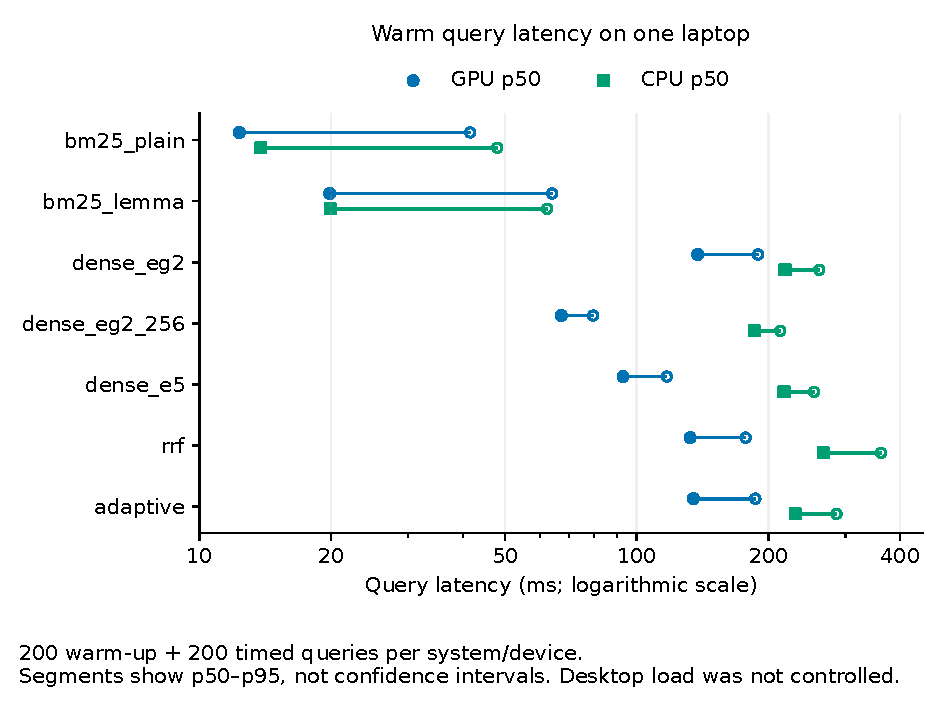
\includegraphics[width=\linewidth]{query_latency.pdf}
\caption{Затримка запитів після повного розігріву. Маркери показують p50, відкриті кінці --- p95, а не довірчі межі; горизонтальна вісь логарифмічна. Обидва прогони включають усі 200 запитів.}
\label{fig:query-latency}
\end{figure}

\begin{figure}[p]
\centering
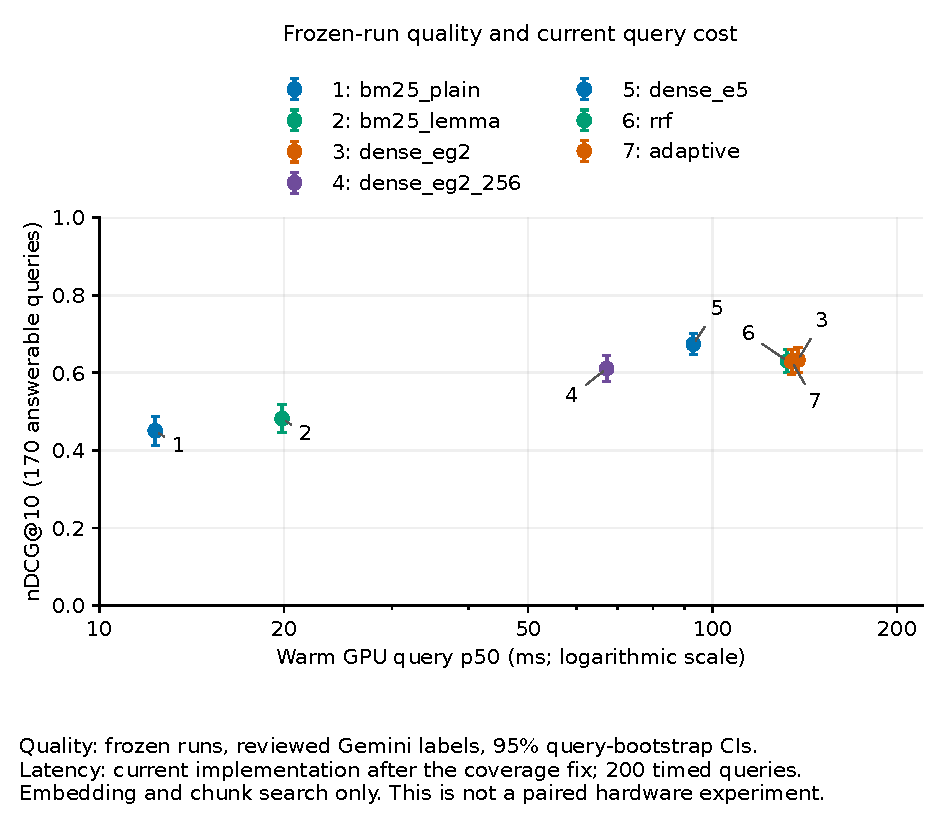
\includegraphics[width=\linewidth]{latency_quality.pdf}
\caption{Якість за початковими зафіксованими прогонами та поточна затримка запиту на GPU після розігріву. Інтервали якості використовують 170 запитів із відповіддю й переглянуті мітки Gemini; затримка --- усі 200 запитів після виправлення покриття цілих слів. Осі описують різні версії коду, як зазначено в контрольному аналізі; це не парний експеримент обладнання. Згортання до документів не входить у таймер.}
\label{fig:latency-quality}
\end{figure}
\else
\pending{Повні вимірювання затримки CPU/GPU}
\fi
\ifpaperindexing
Табл.~\ref{tab:indexing} подає GPU-вибірку з 475 файлів і CPU-вибірку з 95. Їхній склад різний; фрагменти за секунду характеризують ці прогони, а співвідношення повного часу не є парною оцінкою апаратного прискорення.
\begin{table}[p]
\centering
\caption{Індексування в порожню базу двох фіксованих вибірок різного розміру. Кількості стосуються вибраних файлів і створених фрагментів; RSS --- пік дочірнього процесу. Вибіркова БД включає службові файли; розміри повних індексів стосуються основних файлів баз.}
\label{tab:indexing}
% Generated from primary=gemini_reviewed; see ../manifest.json for source SHA-256.
% indexing a fixed sample of the corpus with the archive CLI; source efficiency.json
\begingroup\small\setlength{\tabcolsep}{4pt}\renewcommand{\arraystretch}{1.3}
\noindent\begin{tabularx}{\linewidth}{@{}l*{7}{>{\centering\arraybackslash}X}@{}}
\toprule
Пристрій & Файли & Фрагменти & Секунди & Фрагм./с & БД, МіБ & RSS, МіБ & VRAM +МіБ \\
\midrule
GPU & 475 & 5\,155 & 106.1 & 48.58 & 59.9 & 2591 & 6816 \\
CPU & 95 & 1\,187 & 1395.1 & 0.85 & 13.6 & 2979 & 0 \\
\bottomrule
\end{tabularx}\endgroup

\par\medskip
% main database files; sample disk above includes sidecars
\begingroup\small\setlength{\tabcolsep}{4pt}\renewcommand{\arraystretch}{1.3}
\noindent\begin{tabularx}{\linewidth}{@{}l*{1}{>{\centering\arraybackslash}X}@{}}
\toprule
Повний індекс & Основна БД, МіБ \\
\midrule
e5.sqlite3 & 1096.4 \\
full.sqlite3 & 1120.7 \\
noshort.sqlite3 & 1208.5 \\
plain.sqlite3 & 1094.7 \\
\bottomrule
\end{tabularx}\endgroup

\end{table}
\else
\pending{Повні вимірювання індексування CPU/GPU}
\fi

\subsection{Пошук із квантуванням}
\ifpapergguf
\begin{table}[p]
\centering
\caption{GGUF-збірки EG2 на тих самих текстових кандидатах, що й еталон bfloat16. Затримку виміряно після розігріву всіма 200 запитами. Різниці використовують переглянуті мітки Gemini та дослідницькі некориговані парні тести; неоцінені результати вважаються нерелевантними. Розміри файлів --- МіБ.}
\label{tab:gguf}
% Generated from primary=gemini_reviewed; see ../manifest.json for source SHA-256.
% dense EG2 on the 4137 text documents; labels gemini_reviewed; source efficiency.json quantization
\begingroup\small\setlength{\tabcolsep}{4pt}\renewcommand{\arraystretch}{1.3}
\noindent\begin{tabularx}{\linewidth}{@{}l*{3}{>{\centering\arraybackslash}X}@{}}
\toprule
Збірка & Файл, МіБ & Фрагм./с & Запит p50 \\
\midrule
bf16 (SentenceTransformers) & -- & -- & -- \\
f16 & 532 & 46 & 76.7 \\
Q8\_0 & 296 & 48 & 86.0 \\
Q4\_K\_M & 173 & 46 & 83.6 \\
\bottomrule
\end{tabularx}\endgroup

\par\medskip
% dense EG2 on the 4137 text documents; labels gemini_reviewed; source efficiency.json quantization
\begingroup\small\setlength{\tabcolsep}{4pt}\renewcommand{\arraystretch}{1.3}
\noindent\begin{tabularx}{\linewidth}{@{}l*{4}{>{\centering\arraybackslash}X}@{}}
\toprule
Збірка & nDCG@10 & $\Delta$ [95\% ДІ] & p & Неоцінені@10 \\
\midrule
bf16 (SentenceTransformers) & 0.631 & -- & -- & 0.003 \\
f16 & 0.631 & \shortstack{-0.001 \\ {\footnotesize[-0.005, +0.003]}} & 0.734 & 0.016 \\
Q8\_0 & 0.630 & \shortstack{-0.002 \\ {\footnotesize[-0.006, +0.003]}} & 0.504 & 0.018 \\
Q4\_K\_M & 0.613 & \shortstack{-0.018 \\ {\footnotesize[-0.030, -0.006]}} & 0.002 & 0.099 \\
\bottomrule
\end{tabularx}\endgroup

\par\medskip
% dense EG2 on the 4137 text documents; labels gemini_reviewed; source efficiency.json quantization; unjudged documents removed before ranking evaluation
\begingroup\small\setlength{\tabcolsep}{4pt}\renewcommand{\arraystretch}{1.3}
\noindent\begin{tabularx}{\linewidth}{@{}l*{3}{>{\centering\arraybackslash}X}@{}}
\toprule
Збірка & Condensed nDCG@10 & $\Delta$ [95\% ДІ] & p \\
\midrule
bf16 (SentenceTransformers) & 0.632 & -- & -- \\
f16 & 0.634 & \shortstack{+0.002 \\ {\footnotesize[-0.002, +0.006]}} & 0.297 \\
Q8\_0 & 0.633 & \shortstack{+0.000 \\ {\footnotesize[-0.004, +0.005]}} & 0.869 \\
Q4\_K\_M & 0.636 & \shortstack{+0.004 \\ {\footnotesize[-0.007, +0.015]}} & 0.454 \\
\bottomrule
\end{tabularx}\endgroup

\end{table}
\begin{figure}[p]
\centering
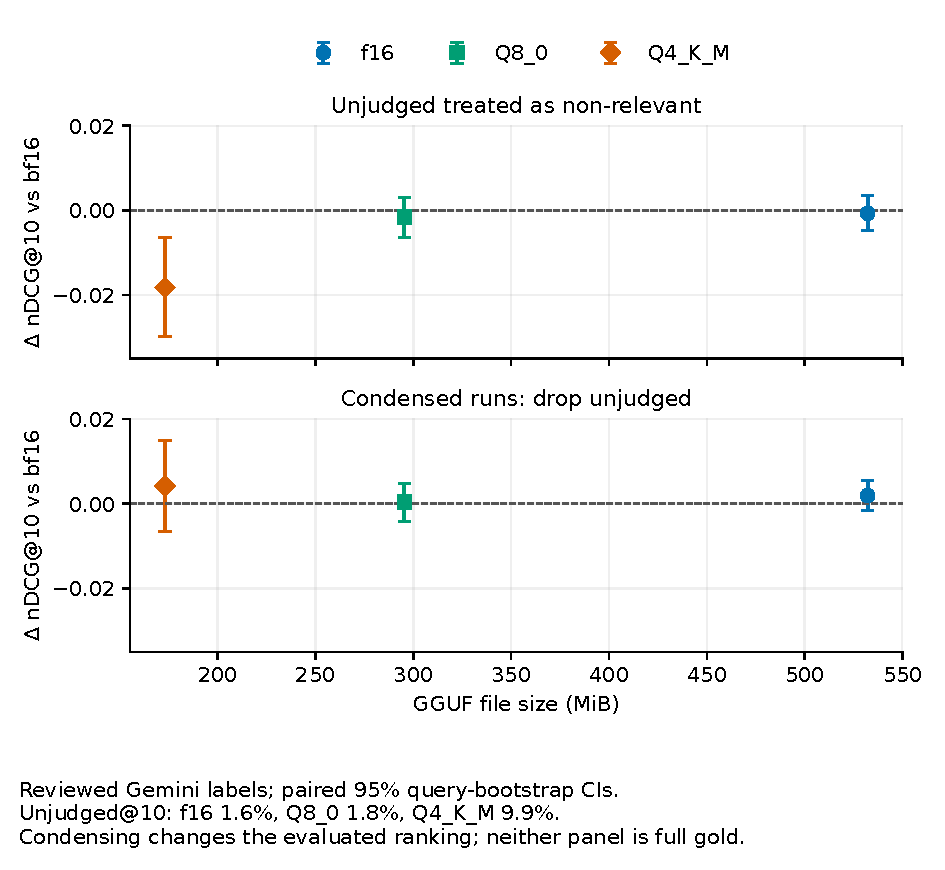
\includegraphics[width=\linewidth]{quantization_quality.pdf}
\caption{Парні різниці nDCG@10 від еталона bf16 EG2 залежно від розміру GGUF на однакових текстових кандидатах. Верхня панель вважає неоцінені документи нерелевантними, нижня --- вилучає їх. Відрізки --- 95\% бутстреп-інтервали за запитами. Залежність від охоплення оцінювання не дозволяє вважати верхню різницю Q4 ізольованим ефектом квантування.}
\label{fig:quantization-quality}
\end{figure}
Табл.~\ref{tab:gguf} показує якість пошуку, швидкість кодування та затримку запиту локального сервера. Окремий косинусний експеримент у додатку не замінює цих пошукових порівнянь. Точкові різниці f16 і Q8 від еталона bf16 малі, але інтервали, що містять нуль, не доводять еквівалентності. Для Q4 трактування неоцінених результатів як нерелевантних дає різницю $-0{,}018$ (95\% ДІ $[-0{,}030,-0{,}006]$); 9,9\% його першої десятки не оцінено проти 0,3\% для еталона. На стиснутих прогонах різниця Q4 становить $+0{,}004$ з інтервалом, що охоплює нуль. Вилучення неоцінених результатів змінює оцінюване ранжування, але не встановлює їхньої релевантності. Отже, зафіксований пул не дозволяє встановити власну втрату якості Q4. Порівняння також змінюють бекенд і числову точність, а не лише квантування.
\else
\pending{Пошуковий експеримент GGUF не завершено; косинусні оцінки наведено в додатку}
\fi

\subsection{Синтетичне масштабування}
\ifpaperann
\begin{table}[p]
\centering
\caption{Точний і наближений пошук на синтетичних колекціях зі справжніх векторів. Затримка --- p50 мілісекунд для одного запиту. Комірки HNSW містять затримку / повноту@10 відносно точного пошуку; час побудови --- секунди. Вимірюється лише пошук векторів фрагментів.}
\label{tab:ann}
% Generated from primary=gemini_reviewed; see ../manifest.json for source SHA-256.
% p50 ms per single query; HNSW cells: p50 ms / strict-ID recall@10 against exact; source ann_scaling.json
\begingroup\small\setlength{\tabcolsep}{4pt}\renewcommand{\arraystretch}{1.3}
\noindent\begin{tabularx}{\linewidth}{@{}l*{5}{>{\centering\arraybackslash}X}@{}}
\toprule
Векторів & NumPy top-k & Faiss flat & Побудова HNSW, с & HNSW ef64 & HNSW ef256 \\
\midrule
100\,000 & 6.16 & 10.65 & 9 & 0.19 / 0.914 & 0.57 / 0.984 \\
300\,000 & 17.85 & 26.52 & 33 & 0.27 / 0.940 & 0.69 / 0.990 \\
1\,000\,000 & 51.78 & 75.83 & 187 & 0.29 / 0.904 & 0.97 / 0.991 \\
2\,000\,000 & 106.63 & 139.95 & 676 & 0.39 / 0.893 & 1.28 / 0.983 \\
\bottomrule
\end{tabularx}\endgroup

\par\medskip
% Actual semantic_scored path with candidate gather, full sort, pool400; no database polling; flat exact agreement / fraction at reference kth score within1e-6; source ann_reference_audit.json
\begingroup\small\setlength{\tabcolsep}{4pt}\renewcommand{\arraystretch}{1.3}
\noindent\begin{tabularx}{\linewidth}{@{}l*{3}{>{\centering\arraybackslash}X}@{}}
\toprule
Векторів & Пошук архіву p50, мс & Збіг ID flat & Поріг оцінки flat \\
\midrule
100\,000 & 60.84 & 1.000 & 1.000 \\
300\,000 & 166.80 & 1.000 & 1.000 \\
1\,000\,000 & 497.64 & 1.000 & 1.000 \\
2\,000\,000 & 2441.83 & 1.000 & 1.000 \\
\bottomrule
\end{tabularx}\endgroup

\par\smallskip
На 2\,000\,000 векторах спостережена p50 становить 106.6 мс для оптимізованого NumPy top-k і 2441.8 мс для векторного пошуку архіву. HNSW ef256 має 1.28 мс за повноти@10 за ідентифікаторами 0.9825. Це послідовні вимірювання різних алгоритмів і розмірів видачі (10 проти 400) у робочому сеансі, а не парне прискорення обладнання чи наскрізна затримка інтерфейсу.

\end{table}
\begin{figure}[p]
\centering
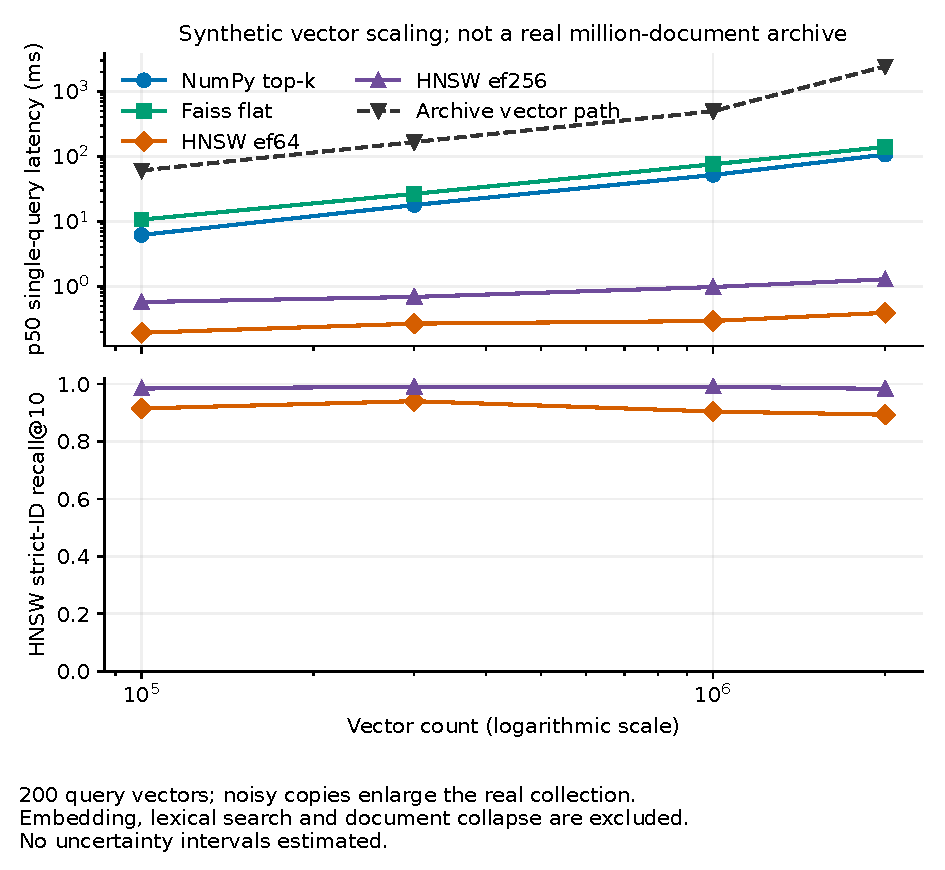
\includegraphics[width=\linewidth]{ann_scaling.pdf}
\caption{Затримка векторного пошуку й повнота HNSW на синтетично збільшених колекціях. Вісь затримки логарифмічна; інтервали невизначеності не оцінюються.}
\label{fig:ann-scaling}
\end{figure}
Табл.~\ref{tab:ann} відокремлює вартість точного векторного пошуку від наближення HNSW. Тут немає кодування запиту, лексичного пошуку та згортання документів; це не оцінка релевантності на справжньому архіві з мільйона документів.
\else
\pending{Повний експеримент масштабування exact/Faiss/HNSW}
\fi

\subsection{Додаткові типи цілей}\label{sec:results-extension}
\ifpaperextension
Окреме розширення містить 50 запитів Qwen до 20 документів, 15 таблиць і 15 файлів репозиторіїв та використовує виправлене правило покриття. Початкові мітки Gemini і Gemma~4 12B подано окремо в табл.~\ref{tab:extension}. 50 записів містять 49 різних формулювань: одне використано для двох файлів. Вони не змішуються з початковими 200 чи їхніми основними мітками релевантності. GPT використовується лише для порівняння. Відмінності між популяціями запитів не ідентифікують самопреференцію, адже також різняться авторство, тип цілі та складність.
\begin{table}[p]
\centering
\caption{nDCG@10 і 95\% бутстреп-інтервали за запитами на окремому розширенні з 50 запитів. Обидва варіанти міток --- початкові оцінки; жоден не є переглянутим основним варіантом початкового тесту.}
\label{tab:extension}
% Generated from primary=gemini_reviewed; see ../manifest.json for source SHA-256.
% nDCG@10, 95% query-bootstrap CI; separate 50-query extension; source extension.json
\begingroup\small\setlength{\tabcolsep}{4pt}\renewcommand{\arraystretch}{1.3}
\noindent\begin{tabularx}{\linewidth}{@{}l*{2}{>{\centering\arraybackslash}X}@{}}
\toprule
Система & Gemini initial & Gemma 12B initial \\
\midrule
bm25\_plain & \shortstack{0.496 \\ {\footnotesize[0.404, 0.590]}} & \shortstack{0.507 \\ {\footnotesize[0.409, 0.604]}} \\
bm25\_lemma & \shortstack{0.523 \\ {\footnotesize[0.431, 0.617]}} & \shortstack{0.540 \\ {\footnotesize[0.443, 0.639]}} \\
dense\_eg2 & \shortstack{0.759 \\ {\footnotesize[0.697, 0.817]}} & \shortstack{0.769 \\ {\footnotesize[0.701, 0.832]}} \\
dense\_e5 & \shortstack{0.721 \\ {\footnotesize[0.654, 0.785]}} & \shortstack{0.730 \\ {\footnotesize[0.666, 0.790]}} \\
rrf & \shortstack{0.684 \\ {\footnotesize[0.619, 0.749]}} & \shortstack{0.696 \\ {\footnotesize[0.623, 0.766]}} \\
adaptive & \shortstack{0.756 \\ {\footnotesize[0.694, 0.814]}} & \shortstack{0.765 \\ {\footnotesize[0.697, 0.827]}} \\
adaptive-phrase & \shortstack{0.756 \\ {\footnotesize[0.694, 0.814]}} & \shortstack{0.765 \\ {\footnotesize[0.697, 0.827]}} \\
adaptive-ident & \shortstack{0.756 \\ {\footnotesize[0.694, 0.814]}} & \shortstack{0.765 \\ {\footnotesize[0.697, 0.827]}} \\
adaptive-short & \shortstack{0.756 \\ {\footnotesize[0.694, 0.814]}} & \shortstack{0.765 \\ {\footnotesize[0.697, 0.827]}} \\
dense\_eg2\_256 & \shortstack{0.713 \\ {\footnotesize[0.639, 0.782]}} & \shortstack{0.732 \\ {\footnotesize[0.662, 0.797]}} \\
\bottomrule
\end{tabularx}\endgroup

\end{table}

За початковими мітками Gemini EG2 має 0,759, адаптивне злиття --- 0,756, E5 --- 0,721, а BM25 із лемами --- 0,523. За початковими мітками Gemma~4 12B відповідні оцінки становлять 0,769, 0,765, 0,730 і 0,540. Адаптивний метод перевершує обидва лексичні базові методи після поправки Holm за обох варіантів міток; ці тести не відокремлюють від нього ні EG2, ні E5. Зміна точкового порядку щільних енкодерів стосується цієї популяції, а не порівняння загальної складності з початковим тестом. GPT лишається найпоблажливішим і на запитах Qwen (середня оцінка 0,550 проти 0,379 у Gemini й 0,437 у Gemma), що підсилює висновок: початковий патерн GPT не ідентифікує самопреференції автора запитів.

\ifpaperextensionunique
Збереження найменшого ідентифікатора для кожного нормалізованого формулювання вилучає q249 без добору за оцінкою пошуку. Табл.~\ref{tab:extension-unique} показує цей дослідницький аналіз чутливості. Інтервали для 50 записів використовують записи як одиниці перевибірки попри спільне формулювання; окремий аналіз усуває цей дублікат, але не робить вибірку репрезентативною.
\begin{table}[p]
\centering
\caption{П'ять основних систем на підмножині унікальних формулювань розширення. Початкові мітки й бутстреп-інтервали за запитами; інші системи та парні статистики збережено в JSON результатів.}
\label{tab:extension-unique}
% Generated from primary=gemini_reviewed; see ../manifest.json for source SHA-256.
Чутливість на унікальних формулюваннях: 49 запитів.
\par\smallskip
% keep lowest qid per normalized wording; source extension.json
\begingroup\small\setlength{\tabcolsep}{4pt}\renewcommand{\arraystretch}{1.3}
\noindent\begin{tabularx}{\linewidth}{@{}l*{2}{>{\centering\arraybackslash}X}@{}}
\toprule
Система & Gemini initial & Gemma 12B initial \\
\midrule
bm25\_plain & \shortstack{0.503 \\ {\footnotesize[0.407, 0.597]}} & \shortstack{0.513 \\ {\footnotesize[0.414, 0.611]}} \\
bm25\_lemma & \shortstack{0.530 \\ {\footnotesize[0.439, 0.624]}} & \shortstack{0.546 \\ {\footnotesize[0.448, 0.646]}} \\
dense\_e5 & \shortstack{0.717 \\ {\footnotesize[0.649, 0.782]}} & \shortstack{0.724 \\ {\footnotesize[0.659, 0.786]}} \\
dense\_eg2 & \shortstack{0.757 \\ {\footnotesize[0.695, 0.813]}} & \shortstack{0.765 \\ {\footnotesize[0.698, 0.826]}} \\
adaptive & \shortstack{0.754 \\ {\footnotesize[0.692, 0.810]}} & \shortstack{0.760 \\ {\footnotesize[0.694, 0.821]}} \\
\bottomrule
\end{tabularx}\endgroup

\end{table}
\fi

\else
\pending{Окреме розширення з 50 запитів до документів, таблиць і коду та його оцінювання}
\fi
